%!TEX root = thesis.tex

%:-------------------------- Preamble -----------------------

% Three languages are supported, which will be reflected in the logo on the front page. Pass the appropriate language
% specified as a class option to uit-thesis. Passing any other languages supported by babel will result in the default
% language on the frontpage. If no language is passed, the default is selected.
%  - USenglish (default)
%  - norsk
%  - samin
% The frontpage comes in two variants, Master's thesis and PhD. Master is default, use classoption 'phd' for the PhD version.
\documentclass[USenglish]{uit-thesis}


% Lorem ipsum
%\usepackage{lipsum}

\makeglossaries

% Add external glossaryentries
\loadglsentries{acronyms}
\newacronym{api}{API}{application programming interface}\glsunset{api}
\newacronym{2api}{2API}{application programming interface}
\newacronym{d3}{D3}{Data-Driven Documents}
\newacronym{html5}{HTML5}{version 5 of the HyperText Markup Language standard}
\newacronym{wsn}{WSN}{Wireless Sensor Network}
\newacronym{bs}{BS}{Base Station}
\newacronym{ch}{CH}{Cluster Head}
\newacronym{coat}{COAT}{Climate-ecological Observatory for Arctic Tundra}
\newacronym{ou}{OU}{Observation Unit}
\newacronym{leach}{LEACH}{Low-Energy Adaptive Clustering Hierarchy}
\newacronym{fleach}{F-LEACH}{Fuzzy-LEACH}
\newacronym{gbcp}{GBCP}{Gossip-based communication protocol}
\newacronym{pegasis}{PEGASIS}{Power-efficient gathering in sensor information systems}
\newacronym{gaf}{GAF}{Geographic Adaptive Fidelity}
\newacronym{gear}{GEAR}{Geographic and Energy-Aware Routing}
\newacronym{tcp}{TCP}{Transmission Control Protocol}
\newacronym{p2p}{P2P}{Peer-To-Peer}
\newacronym{dao}{DAO}{Distributed Arctic Observation}


\newglossaryentry{thesis}
{
  name=thesis,
  description={is a document submitted in support of candidature for an
    academic degree or professional qualification presenting the author's research and findings},
}
\newglossaryentry{lage}
{
  name={long ass glossary entry},
  description={is a long ass entry with a lot of text describing the properties of the glossary entry. Hopefully this spans some lines now.},
}


\newcommand{\listdefinitionname}{My list of definitions}
\newlistof{definition}{def}{\listdefinitionname}
\newcommand{\definition}[1]{%
  \refstepcounter{definition}%
  \par\noindent\textbf{The Definition~\thedefinition. #1}%
  \addcontentsline{def}{definition}
    {\protect\numberline{\thechapter.\thedefinition}#1}\par%
}

\begin{document}

%:-------------------------- Frontpage ------------------------

\title{Peer Observations of Observation Units}
%\subtitle{Subtitle}			% Optional
\author{Camilla Stormoen}
\thesisfaculty{Faculty of Science and Technology \\ Department of Computer Science}
\thesisprogramme{INF-3981 Master's Thesis in Computer Science ... May 2018}
%\ThesisFrontpageImage{example_image.jpg}	% Optional

\maketitle

%:-------------------------- Frontmatter -----------------------
\frontmatter

%\begin{dedication}
%To Leslie.
%Fuck you very much.
%\end{dedication}


%\begin{epigraph}
%\epigraphitem{Simplicity is prerequisite for reliability.}{Edsger Dijkstra}
%\epigraphitem{Beware of bugs in the above code;\\I have only proved it correct, not tried it.}{Donald Knuth}
%\end{epigraph}


\begin{abstract}
What is wrong with the world? Motivation 1-3 sentences, Arch, Des, Imp, Exp 1,2-3 sentences, results and main conclusion.

%The Arctic Tundra in the far northern hemisphere is one of ecosystems that are most affected by the climate changes in the world today. Every year during the winter, COAT deploys several camera traps in eastern Finnmark, Norway to study predator populations.

%This thesis describes a system that ...

%... we develop a prototype of a peer observation for wsns...

%Results show that the system ...
\end{abstract}

\begin{acknowledgement}
%First I would like to thank my main advisor Professor Otto Anshus and co-advisor Associate Professor John Markus Bjørndalen for providing guidance, support, ideas and feedback whenever I needed it through this thesis.

%I want to express my sincerest gratitude to the \textit{Masterinos}. I would not have made it without you guys. 

%I would also like to thanks my parents for encouraging me to take a higher education and supporting me through every decision. At last I would great thanks to my boyfriend
\end{acknowledgement}

\tableofcontents

%\listofdefinition

%\listoflistings

\printglossary
%\printglossary[type=\acronymtype]
%\printglossaries


%:-------------------------- Mainmatter -----------------------
\mainmatter

\chapter{Introduction}
\textbf{FRA CAPSTONE:}
\textit{The Arctic tundra in the far northern hemisphere is challenged by climate changes in the world today and is one of the ecosystems that are most affected by these changes \cite{coat2016}. The \gls{coat} is a long-term research project developed by five Fram Center\footnote{\url{http://www.framsenteret.no/english}} institutions. Their goal is to create robust observation systems which enable documentation and understanding of climate change impacts on the Arctic tundra ecosystems. COAT was in autumn 2015 granted substantial funding to establish research infrastructure which allowed them to start up a research infrastructure during 2016-2020[10].}


\gls{wsn} is a system that consists of hundreds or thousands of low-cost micro-sensor nodes. These nodes monitor and collect physical and environmental conditions. The various activities  in the sensor nodes consume lots of energy and the battery of the sensor node is difficult to recharge in wireless scenarios and also because the sensor nodes are located at remote areas in the Arctic tundra.

%\Gls{wsn}s main task is to periodically collect information of the interested area and broadcast the information to a \gls{bs}. An easy approach to achieve this task is to make each sensor node transmit their data directly to the BS. But the problem  is that the BS can be far away from the sensor node and the sensor node will die due to energy consumption.

%It is beneficial to make these sensors as cheap and energy-efficient as possible.

\textit{This thesis presents the architecture, design and implementation of a peer observation that can observe and accumulate data from in-situ \glsfirst{ou}s.}

\section{Motivation}
The motivation behind this project is...


%This project will develop an approach to 
%\begin{itemize}
%\item Let observation units observe data observed by observation units. 
%\item To gradually accumulate the data to observation units being a DAO Store (there can be multiple DAO Stores depending on user needs).
%\item Do a prototype of such a system focused on three levels of observation units: (i) In-situ observation units being (ii) observed by back-end observation units, being (iii) observed by a DAO Store observation unit.
%\end{itemize}


The purpose is to fetch and accumulate data observed by \gls{ou}s  for further use.

%The observation units to be used for the prototype comprises Observation Unit Processes executing on PCs and/or Raspberry Pi.


\section{Contributions}
The dissertation makes the following contributions:
\begin{itemize}
\item An introduction to \gls{wsn}s and routing techniques in \gls{wsn}s.
\item An implementation and description of a system ...
\item An evaluation of the system.
\item Thoughts on future work and further improvements to the current system.
\end{itemize}

\section{Assumptions}
Avgrense viktig!

\section{Limitations}
Avgrense viktig!
%Fokus på cluster som tar hensyn til batteri mtp at nodene er ute i tundraen og ikke har mye tilgang til strøm.. redundancy, reliability, scalability?? 
%\paragraph{A paragraph}

\section{Outline}
This thesis is structured into X chapters including the introduction.

\begin{description}
\item[Chapter 2] describes different routing and communication protocols in \gls{wsn}s.
\item[Chapter 3] presents related work in the field of \gls{wsn}, node communication and comparing it to the work done in this thesis.
\item[Chapter 4] describes the technical idea ...
\item[Chapter 5] describes the system architecture.
\item[Chapter 6] describes the design of the system, and shows ...
\item[Chapter 7] describes the implementation of the system together with choices and issues during implementation.
\item[Chapter 8] Evaluation
\item[Chapter 9] discusses the results etc ..
\item[Chapter 10] concludes the thesis.
\item[Chapter 11] suggests future work to improve the system.
\item[Chapter 12] Appendix
\end{description}


%\subsection{A subsection}
%We can use the \ac{api} to \ac{2api} do stuff, and write about what we did in a \gls{thesis}!

%This is some stuff, {\sc smallcaps {\em smallcapsemphasized}} {\em regularemphasized}

%\Gls{lage}: a test glossary entry.

%If the acronym \ac{uit} is displayed, then loadglsentries works.

%It is fun to use modern \upsc{OpenMP} technology!\footnote{This is a snarky footnote. Words and etc. Semantic web technologies are technologies that enable semantification of the Web as we know it today. Hopefully this spans some lines now.}

%It is fun to use \emph{modern \upsc{OpenMP}} technology! And it is fun to use \ac{d3} and \ac{html5}.

%\definition{Some other definition}



\chapter{Routing Techniques in WSNs}
%\textit{Har også fra WSN-bok ("Protocols and Architectures for Wireless Sensor Networks, Holger Karl, Andreas Willig) kap. 11 som heter "Routing Protocols" som sier noe om gossiping, energ-efficient unicast, broadcast/multicast, geographic routing og mobile nodes..}

\gls{wsn} is a system that consists of hundreds or thousands of low-cost micro-sensor nodes which monitor and collect physical and environmental conditions. Figure \ref{fig:wsn} shows how a \gls{wsn} architecture can be. 

\gls{wsn}s  main task is to periodically collect information of the interested area and broadcast the information to a \gls{bs}. An easy approach to achieve this task is to make each sensor node transmit their data directly to the BS. But the problem is that the \gls{bs} can be far away from the sensor node so a direct data transmission would not be possible, or if the routing path from the sensor node to the \gls{bs} is long, the sensor node may require for more energy than available. There are multiple hierarchical protocols that has been proposed as a solution to this problem.

\begin{figure}
\centering
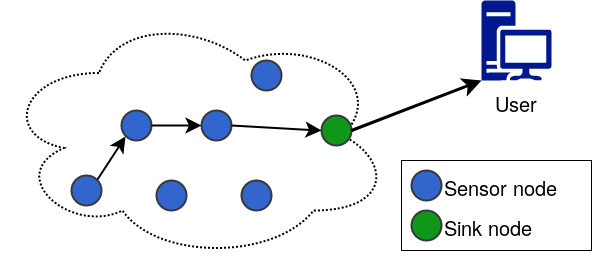
\includegraphics[width=\textwidth]{wsn.png}
\caption{Figure shows an example of a multi-hop \gls{wsn} architecture.}
\label{fig:wsn}
\end{figure}

%\newpage

\section{Routing Protocols in WSNs}
\subsection{Hierarchical Routing}
Hierarchical routing, also called cluster-based routing, is a well know technique for network routing with special advantages related to scalability, efficient communication and lower energy consumption in WSNs. Each cluster in the hierarchical routing protocol have a special node which is responsible for coordinating data transmission between all nodes in the cluster \cite{leach, leach_perf, routing_survey}.

%\textit{Hierarchical routing is an efficient way to lower energy consumption within a cluster, performing data aggregation and fusion in order to decrease the number of transmitted messages to the \gls{bs}.}

Two approaches based on hierarchical routing are \gls{leach}\cite{leach} and \gls{pegasis}\cite{pegasis} which are described in Chapter \ref{chap:related_work}.


\subsection{Location-based Routing}
In location-based routing, are nodes addressed based on their location. The distance between a node's and its neighbour can be estimated by incoming signal strengths, by GPS or via coordination among nodes \cite{routing_survey}. Two approaches are \gls{gaf}\cite{gaf} and \gls{gear}\cite{gear}.


\section{Flood And Gossiping Protocol}
\subsection{Flooding Protocol}
The simplest forwarding rule is to flood the network. In flooding, a node sends a packet received to all its neighbours expect the neighbours which sent the packet until the packet arrives at the destination or maximum number of hops for the packet is reached. Its biggest drawback is that protocol is not an energy efficient protocol and is not designed for sensor networks \cite{wsnbook}.

\subsection{Gossiping Protocol}
Gossiping is a modified version of flooding attempting to correct some of its drawback. In gossiping, a node with updated data will contact an arbitrary node. However, it is possible that the contacted node was updated by another node and in that case may not spreading the update any further \cite{dsbook}.


\chapter{Related Work} \label{chap:related_work}
%\section{Routing Protocols in WSNs}
To improve the overall energy dissipaton of \gls{wsn}s, \gls{leach} \cite{leach} introduce a hierarchical clustering algorithm for sensor networks. It is self-organized and use randomization to distribute the energy load evenly among the sensors in the network. The sensor nodes organize themselves into local clusters where one node is the local \gls{bs} or \gls{ch}. The \gls{ch} are not fixed to avoid nodes to drain their battery and to spread the energy usage over multiple nodes. The nodes self-elect a new \gls{ch} depending on the amount of energy left at the nodes at different time-intervals. \gls{leach} is divided into different rounds where each round include a setup phase and a steady-state phase \cite{tree_based}. In the setup phase will each node decide whether to become a \gls{ch} or not. When a \gls{ch} is chosen, each node will select its own \gls{ch} based on the distance between the node and the \gls{ch} and join the cluster. In the steady-state phase will the \gls{ch} fuse the received data from the node members in the cluster and send it to \gls{bs}.

In contrast, will nodes in our approach first connect to a cluster and then start a \gls{ch} election rather than elect a \gls{ch} first and then nodes joining the cluster. %This is described further in Section/Chapter \ref{xx}.
A resemblance between the two approaches is that neither of them consider a node's energy level when calculating the \gls{ch}.
%\begin{equation}
%T(n) = \frac{P}{1-P\times(r \bmod \frac{1}{P})}
%\end{equation}

%\begin{equation} \label{eq:leach}
%T(n) = \begin{cases}\frac{P}{1-P\times(r \bmod \frac{1}{P})} & if n \in G
%\\0 & otherwise\end{cases}
%\end{equation}


\gls{leach} do not consider a node's energy level when calculating the \gls{ch}. It has therefor been a benchmark for improving algorithms such as the centralized clustering algorithm LEACH-C \cite {leach_c} and distributed clustering algorithm such as LEACH-E \cite{leach_e} and LEACH-B \cite{leach_b}. They concentrate on energy consumption reducing a nodes residual energy and more relevant criterions \cite{dec_cb_alg}.


%\begin{equation} \label{leach_c}
%P_{i}(t)=\min\left\{\frac{E_{i}(t)}{E_{total}(t)}k, 1\right\}
%\end{equation}

\Gls{fleach} \cite{fuzzy_logic, ch_fuzzy} have three different fuzzy descriptors such as energy, concentration and centrality used to complement the cluster head selection process. The \gls{bs} performs the \gls{ch} election in each round by computing the chances of a node becoming a \gls{ch} by calculating the three fuzzy descriptors. \Gls{fleach} also assumes that the \gls{bs} elects the appropriate \gls{ch} because it has a complete information about the whole network.

In contrast to \gls{fleach}, our approach will elect a \gls{ch} by the nodes in the cluster and not in a \gls{bs}. The \gls{ch} election will not consider "variables" such as battery level or number of nodes in the cluster.


\Gls{pegasis} is a chain-based protocol with the idea to form a chain among the sensor nodes so each node will receive and transmit data to a close neighbor. The sensor nodes will also take turns on being the leader for transmitting data to the \gls{bs} and therefor distribute the energy load evenly among the sensor nodes. The chain can be organized by the nodes themselves using a greedy algorithm starting from some node or the \gls{bs} can compute the chain and broadcast it to all the nodes in the network \cite{pegasis}.

To increase the robustness of devices and lower power consumptions, ZebraNet \cite{zebranet} provides a low-power wireless system for position tracking of wildlife by using peer-to-peer network techniques. This reduces the researchers effort to manage the sensors and collecting logged data for their research. The radios on their devices also operates on different frequencies and have different bandwidth, range and other characteristics.

A diversity to our approach is that ZebraNet stores multiple copies of the same data across multiple nodes while our approach forwards the data to the next node in the path to leader. They've also deployed their sensors on zebras in a real-life environment. For us, it's not feasible to deploy sensors out in the real-life Arctic Tundra in such an early development.

%Compared to our approach, 
%ZebraNet stores multiple copies of the same data across multiple nodes whilist our apporach forward the data to a node which is believed to have the best chance to access a base station..


%"When network nodes have multiple radios, the shortest path algorithm does not perform well". p.1 in paper


%\section{Data Collection/Aggregation in WSNs}
%Di Franscesco et. al. \cite{dataColl}


%\section{Gossip-based Protocols}
Gossip-based protocols, or epidemic protocols, are popular protocols due to their ability to reliably pass information among a large set on interconnected nodes. Jelasity et al. \cite{gbsampling} provide a \gls{gbcp} where each node have peers to gossip with in a large-scale distributed system \cite{demers}. These nodes can quickly join and leave the network at any given point of time. The general principle of their framework is that every node (1) maintains a relatively small local membership table that provides a partial view of all nodes and (2) periodically refreshes the table using a gossiping procedure.

The difference between \gls{gbcp} and our approach is that our approach does not use a gossip protocol to update its table of nodes, but instead relies on the communication with other nodes to know about the election of a new \gls{ch}, which of the node is the \gls{ch} and when a node should accumulate data and send it to the \gls{ch}.


\chapter{Idea} \label{chap:idea}
%Technical idea

%Unstructured p2p network..
%Multi-hop communication (not single-hop)

%(Unstructured peer-to-peer networks do not impose a particular structure on the overlay network by design, but rather are formed by nodes that randomly form connections to each other. (Gnutella, Gossip, and Kazaa are examples of unstructured P2P protocols), the role of all peers in the network is the same, unstructured networks are highly robust in the face of high rates of "churn"—that is, when large numbers of peers are frequently joining and leaving the network

%Decentralized- no single point of failure. but coordinators can crash..
%Centralized - Partially centralized: supernodes act as local central indexes, some nodes assume a more important role

%hva er veien, ikke hvilken vei..

The technical idea behind the system is that it should be a partially centralized unstructured \gls{p2p} system where nodes, also called \gls{ou}s, connect to nearby nodes and create clusters. Using a unstructured network would be efficient to use when large number of nodes are frequently joining and leaving the network since its highly robust in the face of high rates of churn.

In a partially centralized network are the role of all peers the same except of some nodes that assume a more important role. These nodes are called \gls{ch}s or super nodes. These \gls{ch}s will be important when accumulating data for further use. A node will assume a more important role in the network by sub-factors discussed in Section \ref{disc:ch_election}.

All nodes should be able to observe data observed by other nodes and to gradually accumulate data to \gls{ou}s being a a \gls{ch} or e.g. a \gls{dao} Store.

Since it is not feasible to deploy nodes in the Arctic Tundra at such an early development, there should be a functionality to make nodes discover nearby nodes they can connect to as similar to a real-life environment.

The technical idea is shown in Figure \ref{fig:idea}.

\begin{figure}
\centering
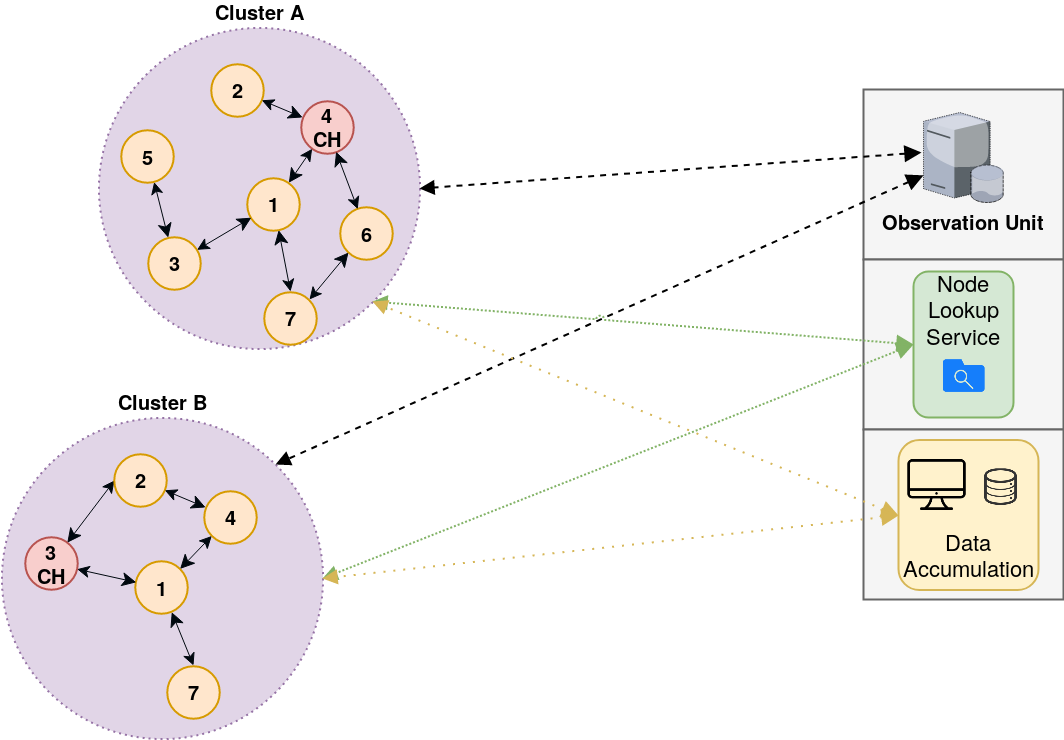
\includegraphics[width=\textwidth]{idea.png}
\caption{Figure shows the architecture of the system.}
\label{fig:idea}
\end{figure}


\chapter{Architecture}
%Tell it clean/neat. Abstractions, functionalities

This chapter describes the architecture of the system. The main functionality can be divided into 4 sub-sections: a nodes lookup service, discovery of other nodes, data accumulation and incoming- and outgoing network requests. The architecture of the system is presented in Figure \ref{fig:architecture3}.


\begin{figure}
\centering
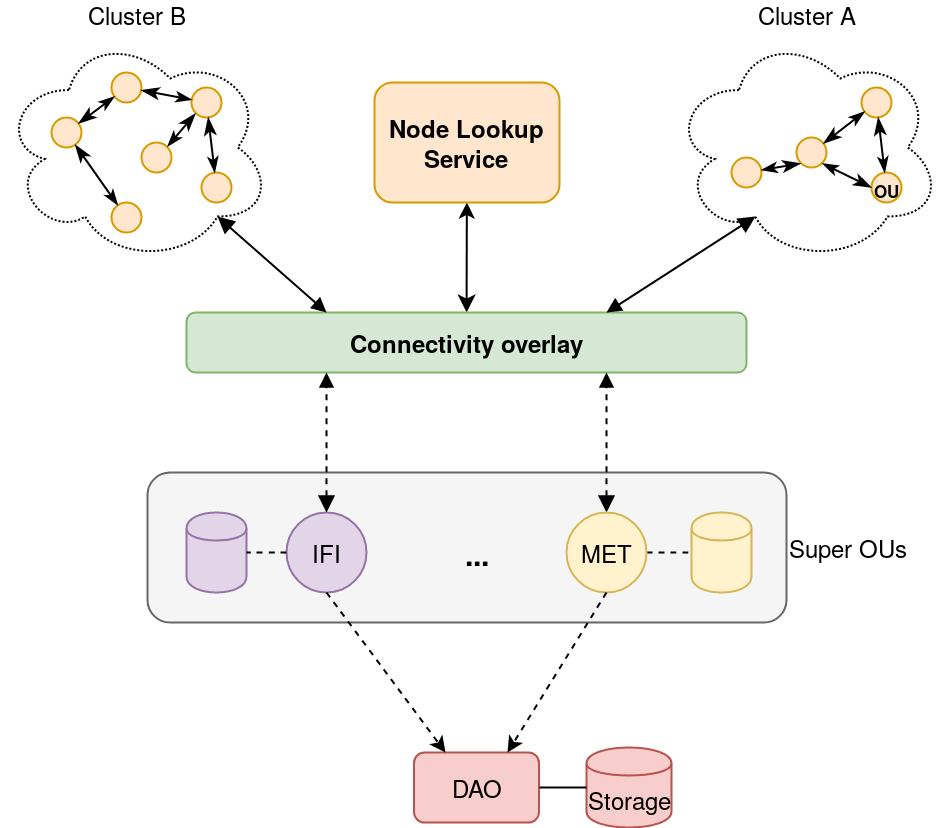
\includegraphics[width=\textwidth]{arch3.png}
\caption{Figure shows the architecture of the system.}
\label{fig:architecture3}
\end{figure}

\section{Node Lookup Service} \label{sec:nodeLS}
The lookup service is responsible for storing all previous discovered nodes and their address. This lookup service is responsible for detecting which nodes that are in range for other nodes and return this result to a corresponding node. 

%Hvordan forlkare at det er en egen service som "simulaerer" range??


\section{Discovery Of Other Nodes} \label{sec:discON}
Each node can only discover other nodes within a simulated radio range. Figure \ref{fig:broadcast_range} shows how a simulated radio range of a node may be discovered. When a new node in the network has been discovered, meta-data about the node such as address be stored locally on the node in the cluster.


\section{Data Accumulation}
A node will accumulate data received from another node if its data hasn't been sent to the \gls{ch}. A \gls{ch} will gather data from nodes in order to provide the accumulated data to a \gls{bs} for further use.


\section{Incoming And Outgoing Network Requests}
A node may receive incoming requests from other nodes in the network. The request handler will handle the request based on the type of request. The types of requests a node may receive are listed below.

\subsection{Connect To Neighbours}
When a node receive a list of neighbours in range from the lookup service, it will try to connect to the neighbours that are within the nodes range. It will only connect to the neighbour node if it receives a OK-message, i.e. the node is allowed to connect.

\subsubsection{Receive OK From Neighbours}
When a node receives a OK-message it will connect itself to the neighbour. The neighbour will also then be connected to the new node.

\subsection{Cluster Head Election Request}
When a node receives a \gls{ch} election request it will perform a leader election and forward the result to it's neigbours which will do a leader election as well.
A node may receive a \gls{ch} election request when a node has joined the cluster.

\subsubsection{Cluster Head Election Calculation Request}
If there is a leader in the cluster already and a new election should be proposed, a \gls{ch} election calculation request is sent from the leader. Nodes receiving this request will calculate their \gls{ch} election number. %This is explained further in Section xx.

\subsection{Data Transmission}
\subsubsection{Notify Neighbours About Sending Data To Leader}
A node may receive a request that it should send its data to the leader. This request is forwarded to the nodes neighbour and so on.

\subsubsection{Send Data To Leader}
This request forwards a nodes data to the next node in the path to the leader. If the nodes data receiving this requests isn't sent to the leader of the cluster, will the data be accumulated with the received data and then forwarded to the next node.

%\section{Base Station Access}
%CH should access BS..?


\chapter{Design}
%Server, p2p, protocols..
In this chapter we will look at the design of the system and present the design of each component. Figure \ref{fig:design} shows how the cluster network may appear in the system. Nodes are connected to other nearby nodes represented by arrows and together they form a cluster network.

\begin{figure}
\centering
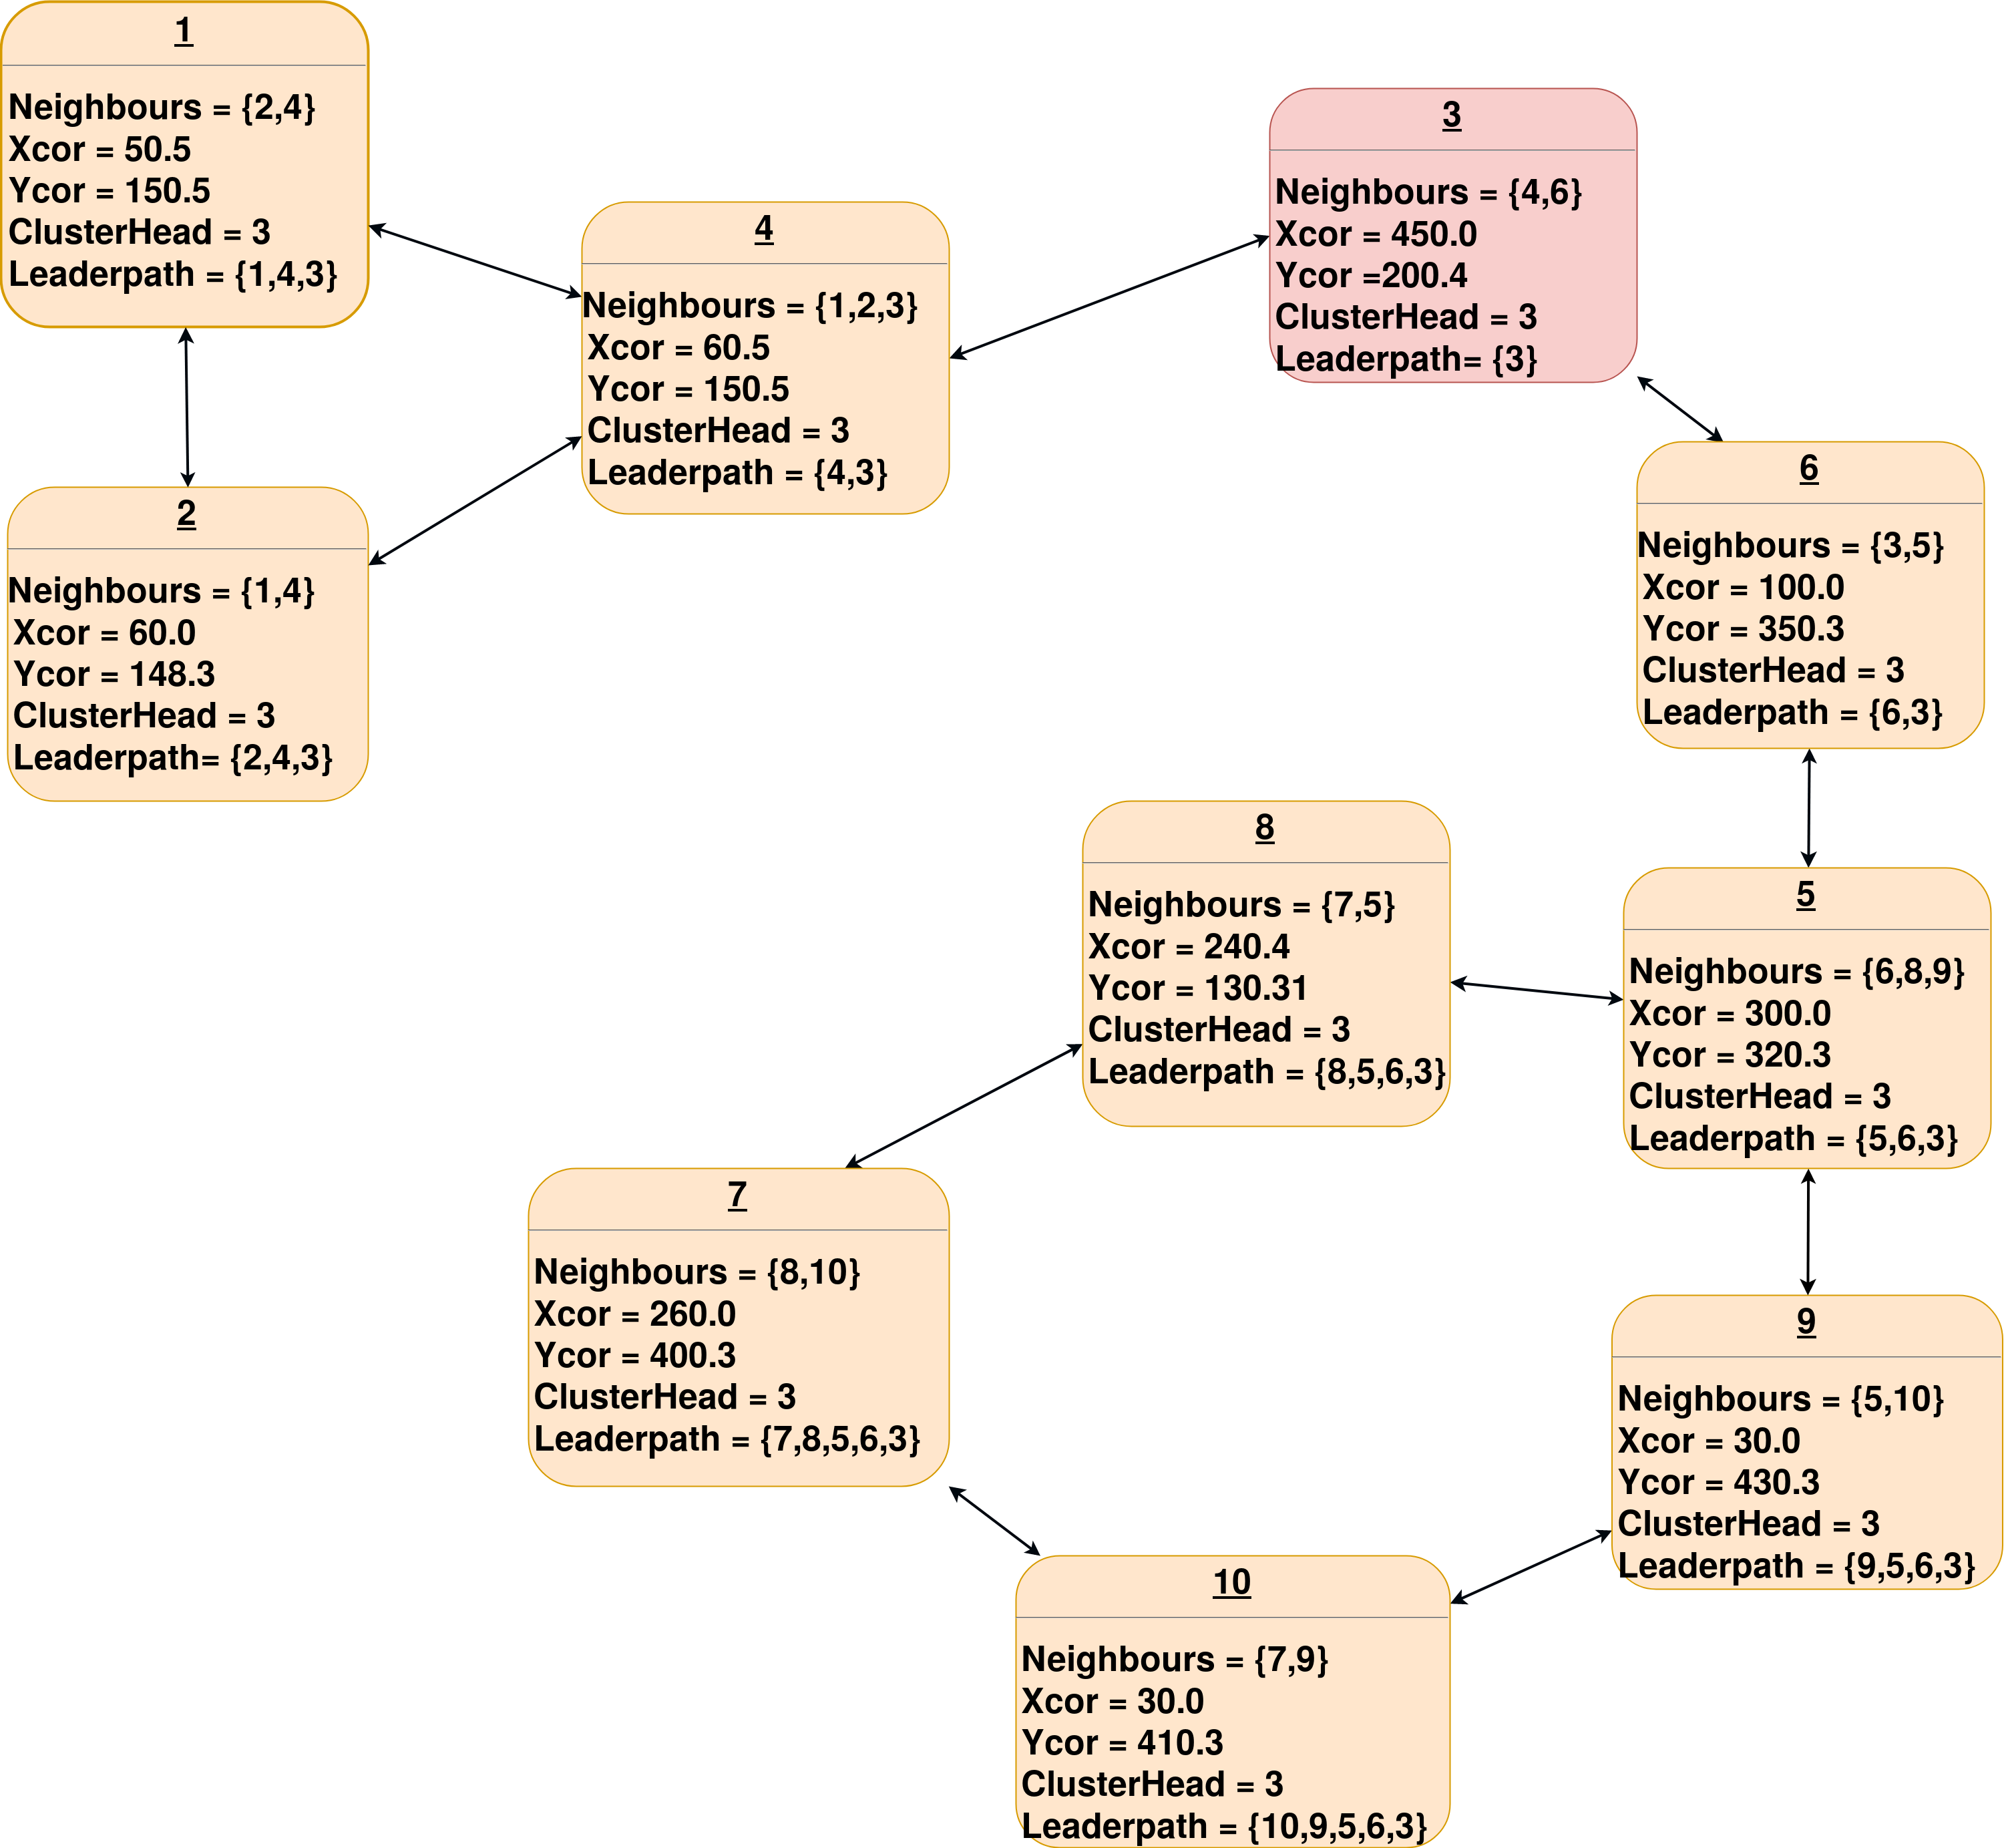
\includegraphics[width=\textwidth]{design.png}
\caption{Figure show design of the system.}
\label{fig:design}
\end{figure}

%\newpage

\section{Discovery Of Other Nodes}
\subsection{Broadcasting}
When a new node start, it will contact the node lookup service to discover other nodes in the network. The node will then initiate a broadcast.
Broadcast is limited due to a radio range limitation where only nodes that are within this range will receive the broadcast, shown in Figure \ref{fig:broadcast_range}. \textit{Node 1} will only reach \textit{node 5} and \textit{node 7}.


\begin{figure}
\centering
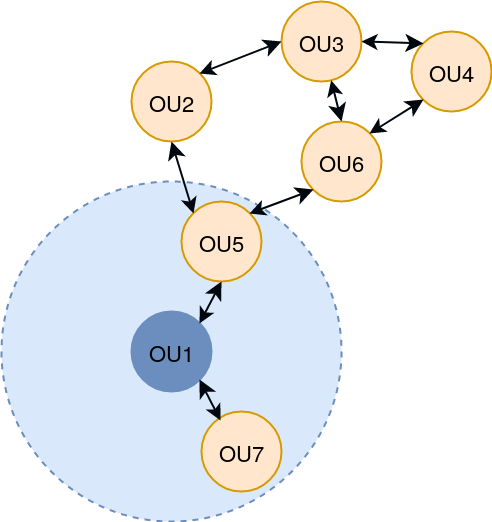
\includegraphics[scale=0.4]{broadcast_range.png}
\caption{Figure show broadcast range of a \gls{ou}.}
\label{fig:broadcast_range}
\end{figure}


%\begin{figure}
%\centering
%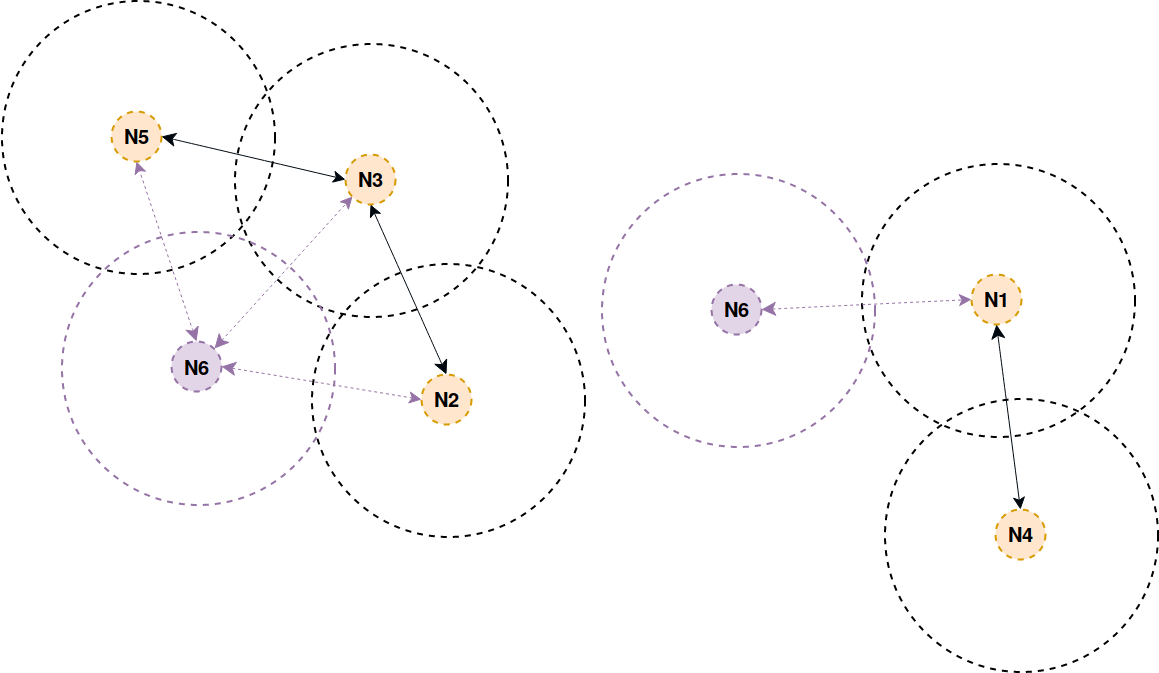
\includegraphics[width=\textwidth]{contactNewNeighbour.png}
%\caption{Figure show how new nodes (purple) contacts their neighbours.}
%\label{fig:contactNeighbour}
%\end{figure}

\newpage

%\section{Maintenance Of Known Nodes}
\section{Cluster Head Election} \label{des:ch_election}
A \gls{ch} election may occur in two scenarios listed below.

%\begin{figure}
%\centering
%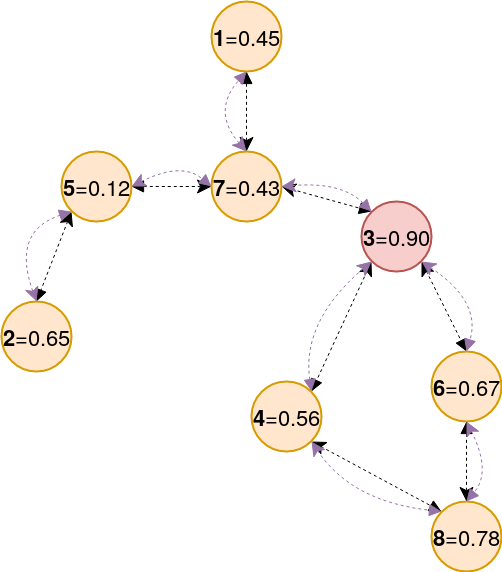
\includegraphics[width=\textwidth]{leaderElection.png}
%\caption{Figure show how a \gls{ch} election is gossiped in the cluster.}
%\label{fig:leaderElection}
%\end{figure}


\subsection{New Node In Cluster Starts Election}
When a new node has joined the cluster, it will start a new \gls{ch} election based on the Bully algorithm. It will calculate it's own \gls{ch}-score and gossip the score to its neighbours. The neighbours will then start a \gls{ch} election comparing the received \gls{ch}-score against their own \gls{ch}-score. The result of the \gls{ch} election will then be gossiped to the node's neighbours with either the received \gls{ch}-score or the nodes own \gls{ch}-score. The gossiped message also contains a path to the leader. The node append its own address to the path if the received \gls{ch}-score won the election, otherwise will the path to leader only contain the node itself. Eventually a new \gls{ch} is elected by all the nodes and the \gls{ch}-election result will be consistent in the whole cluster. An example of a \gls{ch} election is shown in Figure \ref{fig:newNodeLeaderElection}.

\begin{figure}
\centering
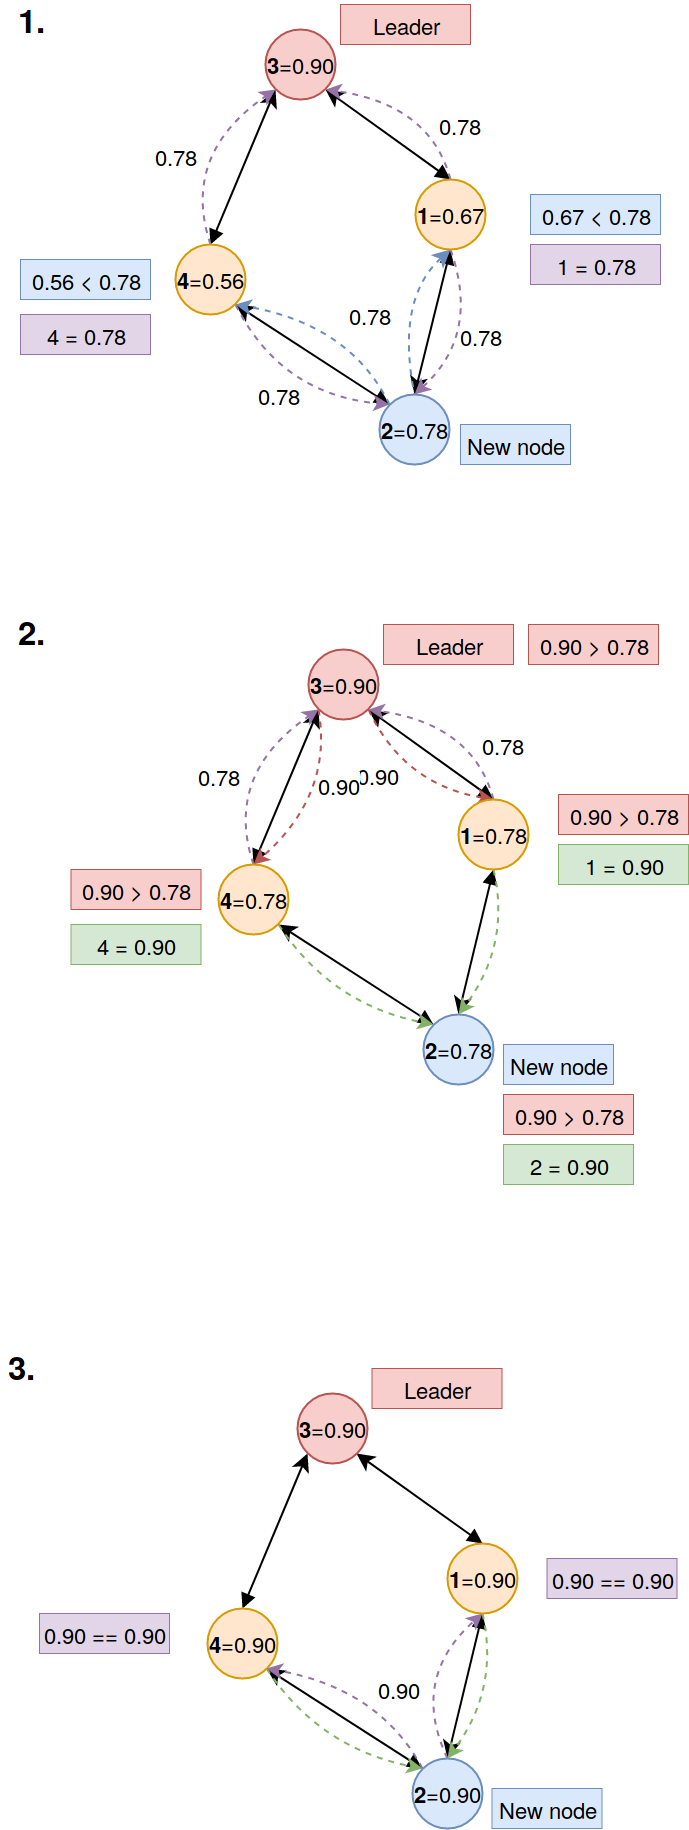
\includegraphics[scale=0.3]{newNodeLeaderElection.png}
\caption{Figure show how a new node starts a leader election.}
\label{fig:newNodeLeaderElection}
\end{figure}

\newpage 

\subsection{Cluster Head Starts Election}
When a \gls{ch} has accumulated data 'X' times, it will start a new \gls{ch} election. Initially, the \gls{ch} will gossip a message to nodes the cluster to calculate a new \gls{ch}-score. Then will the \gls{ch} start a new election and gossip this election to the other nodes. The nodes receiving this gossip message will start their leader-election as described in the section above. The election is illustrated in Figure \ref{fig:chWantsLeaderElection}.

\begin{figure}
\centering
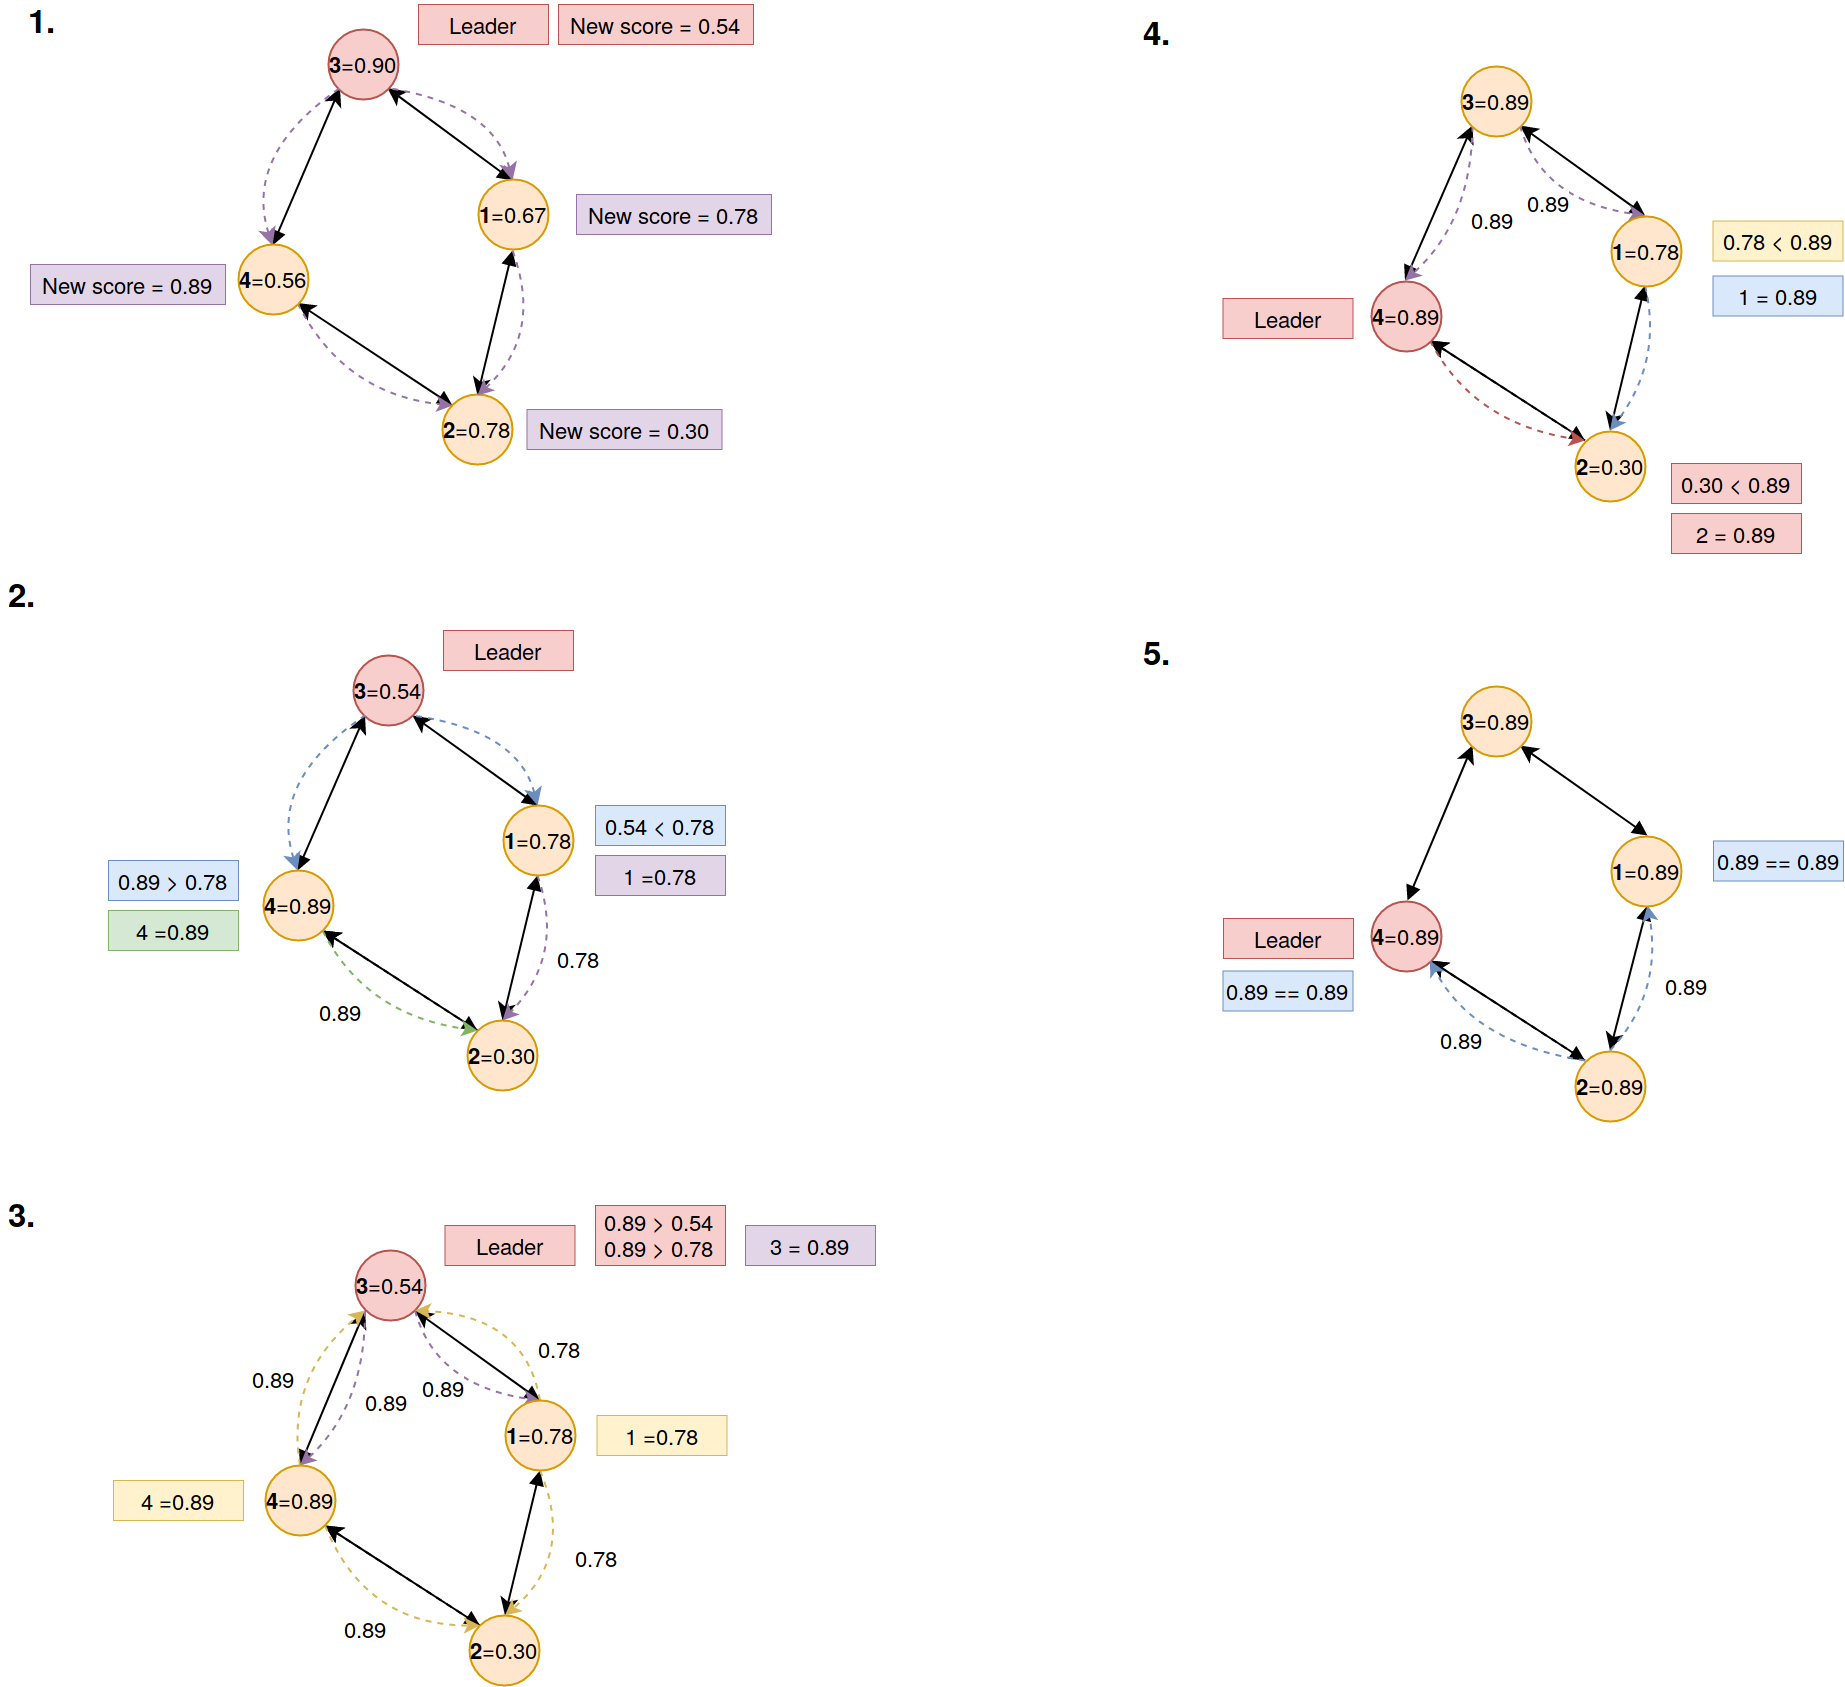
\includegraphics[width=\textwidth]{LeaderNewLeaderElection2.png}
\caption{Figure show how a \gls{ch} starts a leader election.}
\label{fig:chWantsLeaderElection}
\end{figure}


\newpage

\section{Data Accumulation}
A \gls{ch} will start gathering data by gossiping a message to nodes in the cluster, illustrated as the red arrows shown in Figure \ref{fig:gaterSendData}. When a node receives this message it will send its data to the next node in the path to the \gls{ch} as Figure \ref{fig:gaterSendData} shows. When a node receive data from another node it will check if it's own data has been sent to the \gls{ch} or not by a fingerprint and a status. If it hasn't been sent earlier, the node will accumulate the received data with its own data, and then send the data to the next node in the path to \gls{ch}. The \gls{ch} will accumulate all received data and store it.

%A node may at times forward data to another node in the cluster.
%\centering
%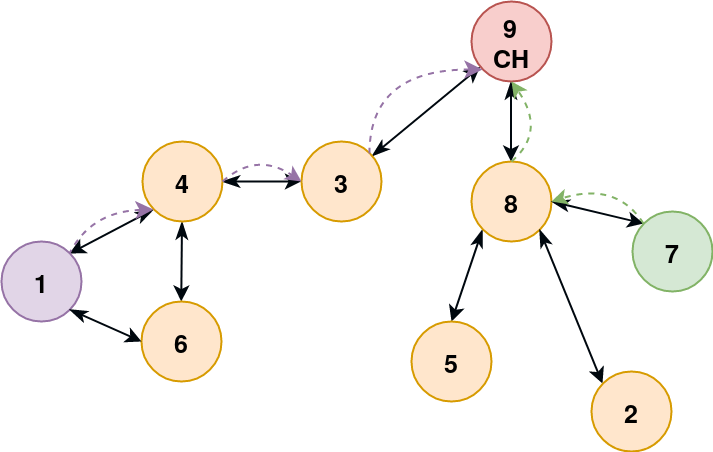
\includegraphics[width=\textwidth]{sendData.png}
%\caption{Figure show how a node sends its data to the leader through the nodes the path.}
%\label{fig:sendData}
%\end{figure}

\begin{figure}
\centering
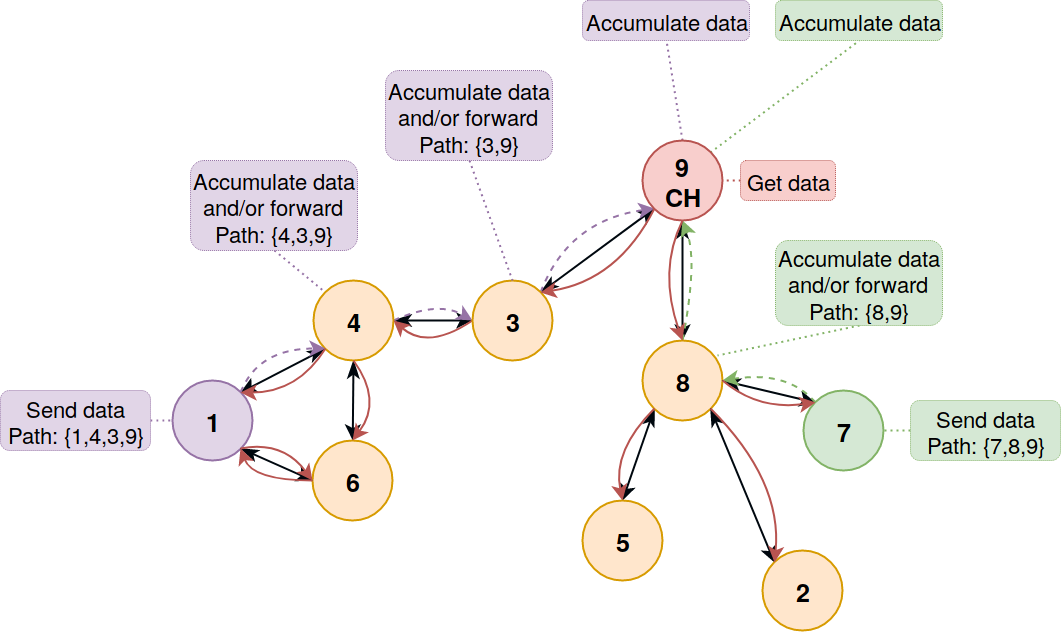
\includegraphics[width=\textwidth]{gatherSendData1.png}
\caption{Figure show how \gls{ch} gossips a GET-data request and how  nodes sends their data to the leader through the nodes in the path.}
\label{fig:gaterSendData}
\end{figure}

%\section{Base Station Access?}
%CH will keep data and send it to BS when it has access??
%CH changes so not


\chapter{Implementation}
%Threads, data structures, language

This chapter will elaborate on how we implemented the system, general implementation requirements, issues and choices. 
%We will first look at some libraries used in this implementation, then we will take a look at ... At last, we will describe the ...

The system is implemented in the open source programming language GO 1.9.3\footnote{\url{https://golang.org/}} and the nodes communicate with each other by Golangs HTTP Server which listens on the \gls{tcp} network. This was a practical choice because we were familiar with the language from previous projects, its developed for making concurrent mechanisms easy and to get the most out of multicore and networked machines, and offers multiple different libraries.

It is not suitable to have nodes deployed in the Arctic Tundra at such an early development. This implementation simulates a real-life environments where nodes can communicate with each other through the \gls{tcp} network. Each node is assigned \textit{x,y} coordinates within a network grid size and a broadcast width.


\section{Distance To Other Nodes In The Network}
A new node will contact the lookup service to discover other nodes in the network by sending a POST-request containing meta-data about itself such as address and position (\textit{x,y} coordinates).

The distance formula \ref{eq:distance}, also called Euclidean distance, is used to calculate the range between two points in a two-dimensional coordinate map and is used to see if a node is within a simulated radio range or not, as seen in Figure \ref{fig:broadcast_range}. The two points to be calculated is the node itself together with all the running nodes in the network.

\begin{equation} \label{eq:distance}
d = \sqrt{(X_{2} - X_{1})^{2}+(Y_{2} - Y_{1})^{2}}
\end{equation}

%node attempt to connect..

Figure \ref{fig:broadcast_simulation} shows how a node contact the lookup service where the node's position is calculated and nodes within the simulated radio range is returned to the node. At last, the node will try to connect to the reachable nodes.

\begin{figure} [!b]
\centering
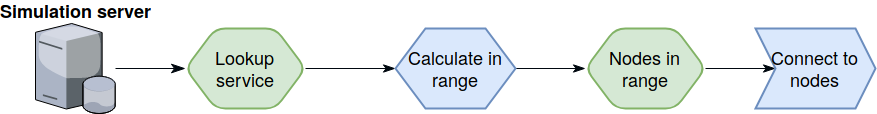
\includegraphics[width=\textwidth]{broadcast_simulation.png}
\caption{Broadcast simulation}
\label{fig:broadcast_simulation}
\end{figure}

\section{Connect To Neighbours}
A node will only be able to connect to another node in the network if the node accept the request to be neighbours. Right now, every node will be able to connect with their neighbours, as long as the node isn't unavailable by means of sleeping or if it's dead. There is no restriction in number of neighbours a node can have or that a node receiving a request from a new neighbour must forward the request to the \gls{ch} and let the leader decide whether the new node can connect to the neighbour or not. Improvements to this approach is discussed in Section \ref{disc:conn_neighbours}.


\section{Cluster Head Election} \label{imp:ch_election}
%Leader election takes time to stabilize because of gossiping..
%Bully algorithm.. traditonially algorithm: nodes ON, we assume nodes OFF/our nodes most likely OFF.. 
%Gossip-based peer sampling - acm - mark jelasity \cite{gbsampling}

%A demo of Dijkstra's algorithm based on Euclidean distance.
A \gls{ch} election is proposed either when a new node joins the network or by a \gls{ch}. 
The \gls{ch} election algorithm is based on the Bully algorithm where the node with the highest ID number is selected to be the leader. Our approach do not use the node with highest ID number, but elect the node with highest score between 0 and 1 to be a \gls{ch}. Each node makes its own decision about whether to become a \gls{ch} or not depending on the received score from neighbour nodes.
Our apporach have several improvements discussed further in Section \ref{disc:ch_election}. 

To avoid flooding the network, each \gls{ch} election round have an ID. If a node receiving an election have received a request with similar ID and the leader haven't changed, the request will not be forwarded to other nodes considering that the node have forwarded the same request previous.


\section{Minimize Path To Leader}
Since \gls{ch} elections are gossiped from all nodes, can each node receive multiple gossip's per \gls{ch} election and some paths will be longer than others. In order to minimize the path to the \gls{ch}, will a node when receiving an election compare its existing path to the one received \cite{dijkstra}.

%Finiding a path to the \gls{ch} is based on Dijkstra algorithm to find the shortest path between two nodes \cite{dijkstra}.

%network traffic, nodes energy/battery, 

%\cite{multiradio}: The goal of the metric is to choose a high-throughput path between a source and a destination.


\section{Data Accumulation}
%fabricated data 

%mediated = try to bring to an agreement

%Fingerprint to identify data and ID to identify packet/msg.. Boolean variable - accumulated..

\subsection{Node Data Accumulation}
Since all nodes run concurrently and independently, can each node receive multiple requests from different neighbouring nodes. When a \gls{ch} creates a request for gathering data, will it contain an ID used for identification. Since the request is gossiped to all nodes in the cluster, a node will most likely receive the same message multiple times, but only need to forward its data once. If a node have not received a request with a specific ID, it will gossip the message to its neighbours and then send its data to the next neighbour in the path to \gls{ch}. Otherwise, the node will just ignore the request.

When a node needs to send data, it will create a request containing the received request-ID from the \gls{ch}, the data to be sent together with a fingerprint and a path to the leader. The path to the leader is a list containing the addresses for the nodes between the sender and the \gls{ch}.

The data is a fabricated byte array with a fingerprint that is the hashed value of the data. The fingerprint will make it easier to identify the numerous data on each node. The data will also have a boolean tag which is used to check whether the data has been accumulated or not.

\subsection{CH Data Accumulation}
As mentioned previous can each node receive multiple requests from different neighbouring nodes.
%Since all nodes run concurrently and independently, can each node receive multiple requests from different neighbouring nodes.
This especially occur in the \gls{ch} when collecting data from the nodes in the cluster. The collected data is stored in a map and maps in Go are not safe for concurrent use. If a map is read from and wrote to from concurrent goroutines, the access must be compromised by a synchronization mechanism. One of the most common ways to protect maps is by using mutexes, illustrated in Listing \ref{test}.

\newpage

\begin{lstlisting} [frame=single,caption={Small Go program showing how mutexes are used when updating a map by CH},language=C, label={test}]

/*SensorData is data from "sensors" on the OU*/
type SensorData struct {
	ID          uint32
	Fingerprint uint32
	Data        []byte
}

/*DBStation is a strucure that contains 
  a map that store data at CH */
var DBStation struct {
	sync.Mutex
	BSdatamap map[uint32][]byte
}

func sendDataToLeaderHandler() {
	var rd SensorData
	
	DBStation.Lock()
	defer DBStation.Unlock()
	
	(...)
	
	err := json.Unmarshal(body, &sData); 
	if err != nil {
		panic(err)
	}
	
	(...)
	
	/*Update map in key FingerPrint
	  with received data */
	DBStation.BSdatamap[rd.Fingerprint] = rd.Data
}
\end{lstlisting}

\newpage

\section{Concurrent CH Election And Data Accumulation}
To avoid having a \gls{ch} election occur concurrently as a data accumulation, are these functionalities scheduled to execute.
Firstly, the \gls{ch} election will execute until the election result is consistent in all nodes. Then will the \gls{ch} broadcast a request for gathering data and nodes will accumulate and send data to the \gls{ch}. After 'X' times gathering data will the \gls{ch} start a new \gls{ch} election. 

%First elect leader, then after a while gather data 'X' times before electing a new leader and so on...
If a \gls{ch} election and a data gathering happens concurrently, there may be issues when the node is supposed to send its data because the \gls{ch} may have changed and the path to the \gls{ch} may be incorrect. This issue and improvements are discussed further in Section \ref{disc:simult_el_acc}.

%If leader election occurs at the same time that a leader is gathering data, get EOF when broadcasting.. But does not stop/exit program..

%\section{Base Station Access}



\chapter{Evaluation}
This chapter describes the experimental setup and metrics used to evaluate the implemented system.

\section{Experimental Setup}
All experiments were done on a Lenovo ThinkCenter with the following specifications:

\begin{itemize} 
\item Intel® CoreTM i5-6400T CPU @ 2.20GHz × 4
\item Intel® HD Graphics 530 (Skylake GT2)
\item 15,6 GiB memory and 503 GB disk
\item Ubuntu 17.04 64-bit with gcc V6.3.0 compiler and GO 1.9.3
\end{itemize}


\section{Experimental Design} \label{eva:exp_des}
%How did we do the experiments?
%For hvert eksperiment bør du prøve å få fram: 
%- hva ønsker du å finne ut? 
%- hvordan måler du + hva måler du? 
%- hva gjør den delen av systemet som du måler? (leser fra disk, regner, sammenligner, koordinerer med andre osv)
%- Hva er metrikken (eks: operasjoner per sekund, minutter per oppgave osv)
%Det gjør det lettere for leseren å henge med. 


%Since it is crucial that the performance cost of running the system is kept to a minimum since it's aimed to execute on small, low-power devices.
%Hvor lenge?? Hvor ofte går testen?

All experiments were conducted on a computer, described in the section \ref{eva:exp_des}, where one process is (executing) one node which is simulating an \gls{ou}. In order to determine how well the nodes perform in terms of memory, CPU and network usage several experiment scenarios were designed and performed, revealing some of the system's capabilities and limitations. It is important that the cost of running the system is kept to a minimum since it's aimed to execute on small, low-power \gls{ou}s.

%Ran with a second's/10th?? measurement interval, system execute normally over X minutes..

simulation shown in Table \ref{tab:simTable}. 

\begin{table}
\centering
\begin{tabular}{|l|l|}
\hline
\textbf{Parameter}       & \textbf{Value} \\ \hline
Number of nodes          & 100            \\ \hline
Network grid size        & 500 x 500      \\ \hline
Node broadcast width     & 100            \\ \hline
\end{tabular}
\caption{Parameters of simulation}
\label{tab:simTable}
\end{table}



\subsection{Memory Measurements} \label{eva:mem_measure}
%needs to be relatively low to enable the device to functi as normal..
We measure the memory usage to discover/observe/see . 


\begin{itemize}
\item \textbf{Psutil - VirtualMemory:} Return statistics about system memory usage.
	\begin{itemize}
	\item \textbf{UsedPercent:} Percentage of RAM used by programs
	\item \textbf{Total:} Total amount of RAM on this system
	\item \textbf{Used:} RAM used by programs
	\end{itemize}	
\end{itemize}


\subsection{CPU Measurements} \label{eva:cpu_measure}
We measure the total CPU usage for 4 cores to discover/observe/see how much computational power is needed to execute the program. 


\begin{itemize}
\item \textbf{Psutil - Percent:} calculates the percentage of CPU used either per CPU or combined.
\end{itemize}


\subsection{Network (Socket) Usage} \label{eva:net_measure}
%psutil - ConnectionPid - Return a list of network connections opened by a process. 
%\subsection{Process Connections Measurements}
%psutil - Process 
%The system relies heavily on network usage and communication between nodes so it is important to measure process connections to keep it to a minimum.

%NUmber of open sockets represent the nymber of communication channels that a device has open at any given point, like discovery request, forwarding and leader election..



\begin{itemize}
\item \textbf{Psutil - Processes:} ???? Process returns a slice of pointers to Process structs for all currently running processes.
\item \textbf{Psutil - ConnectionsPid:} Return a list of network connections opened by a process.
\end{itemize}



\subsection{Network Lifetime?}


\section{Results}
%What does the results say?
In this section we will discuss the results of the testing described in the sections above.

\subsection{Memory Usage}
\subsection{CPU Usage}
\subsection{Network Usage}
%\subsection{Process Connections Measurements}
\subsection{Network Lifetime?}




\chapter{Discussion}
%Idea, arch, design, results, other solutions, "arch has scale issue"..
This chapter discusses our approach, experience, how we solved the problem and why we chose the solution we ended up with..

\section{Availability of nodes in the system}
%ambigious - tvetydig, open to more than one intepretation
%krav

\subsection{Connect To Neighbours} \label{disc:conn_neighbours}
%When a node wants to join the cluster, should it ask the CH or should it join eitherway.. What if CH is sleeping (or busy) so that it's not reachable, or that nodes in the path to CH are sleeping (then how to contact CH?)..

% CH elect if node can join cluster or not...

In the current approach can a node connect to nearby nodes and be a part of a cluster without any restrictions. Another approach would be that when a node receives a request from a new node, it will forward the request to the \gls{ch} which would take the decision if the new node can connect to the cluster or not. However, making a \gls{ch} take this decision could be \textbf{problematic} because the \gls{ch} need to know information about the whole network or at least its own cluster and also need some requirements for when a node can join and not. Some requirements that a \gls{ch} may consider are listed below:

\begin{itemize}
\item Number of nodes per cluster
\item Number of neighbours a node can have
\item Distance from new node to \gls{ch}
\item Node characteristics (bandwidth, energy level, memory etc.)
\end{itemize}

Another interference with having a \gls{ch} take the decision is that the \gls{ch} may be unavailable because it's sleeping or if it's unreachable because nodes in the path to the \gls{ch} are sleeping or unavailable due to e.g. saving battery. 

%Ping othern nodes regulary to check if neighbours are alive or not, or ping right befre a sending of data to ch.. what if a node in the path to leader is dead? what if there is no other way to the ch? what happens? 

A solution to this problem is to ping neighbouring nodes regularly to check if neighbours are alive or not, or to ping neighbours before forwarding a message to the \gls{ch}. This ping-request will most likely contain a wake-up call to the next node in the path to the \gls{ch} so nodes are awake when receiving a forwarding request to the \gls{ch}.

%do not wanna ping to often - flood network?

%However, pinging other nodes frequently will eventually flood the network..

%how to know if node is dead or just sleeping


\subsection{Node Waking Up After Sleeping}
%What if nodes are regulary off/sleep, how to know which one is ch? ask neighbour, and each election have an id/timestamp to check if this is the last election.. Could be that there have been multiple ch electins while node has been asleep so the neighbour node have not the right ch according to other nodes..
%global clock so each node knows when to awake to send data to ch or leader election, etc..?

%Right now: no timestamp or regulation.. If node down, it will send its data to the node he think is the leader, but that is not all bad because data will be send do the leader/gather eventually anyways.. Maybe next round or something.. but improvement: have timestamps or global clock - vector clock..

%Should remember old leader.. or old leader should know that it has been a leader and have data to be sendt to the bs..


What if a node is regularly/often sleeping or off? How to know which one is \gls{ch}?



\section{Cluster Head Election}
%Distance, Power, Availability (Power-Management, Scheduled downtime - repairs etc., network overload)...

%"Being a cluster head is much more energy intensive than being a non-cluster head node. if the cluster heads where chosen a priori and died through the system lifetime, these nodes would quickly use up their limited energy. Once the CH runs out of energy, it is no longer operational, and all the nodes that belong to the cluster lose communcation ability."

Being a \gls{ch} is much more energy intensive than being a regular cluster node because it may transfers data over longer distances and performs more tasks. If the \gls{ch} is chosen a prior would these nodes quickly use up their limited energy. Once a \gls{ch} is runs out of battery, it is no longer operational and all nodes belonging to the cluster will lose their communication ability.

To avoid this problem, will our approach not chose \gls{ch}s a prior. but instead have a leader election algorithm to possibly rotate the \gls{ch}.
%\textbf{possibly/perchance} \textbf{rullere/rotate}


\subsection{Cluster Head Calculation} \label{disc:ch_election}
At the moment, the \gls{ch} election is simply based on which node has the highest score between 0 and 1. Despite the working approach, it does not take in account many other realistic aspects which would improve the \gls{ch} election. To approve this approach and make it more realistic, we could have used several sub-factors listed below:

%now random number, to approve and make it more realistic: 

\begin{itemize}
\item Number of nodes between a node and \gls{ch}
\item Number of neighbours for the node
\item Access to \gls{bs}
\item Power left on node
\item Bandwidth - WiFi, LoRaWan\footnote{\url{https://lora-alliance.org/about-lorawan}}, cable/Ethernet?
\item Prior history
\item Network traffic on node
\end{itemize}

%Bully algorithm.. traditonially algorithm: nodes ON, we assume nodes OFF/our nodes most likely OFF.. 

%\subsection{Eventual Cluster Head Election Consistency?}

\subsection{Gossip Information Between Nodes}
The main advantages of gossiping is its ability to scale. Gossiping have no centralized component where information is coordinated and is therefor an excellent way to rapidly spread information among a large number of nodes using only local information. However, gossiping can not guarantee that all nodes will receive the information \cite{demers}.

To avoid flooding the network, each message sent between nodes have and ID so the node can check if it has received the same message before. If the node have received the message earlier, the node doesn't need to forward the message because it has forwarded the message in an earlier gossip, as described earlier in Section \ref{imp:ch_election}.

Another approach to avoid flooding the network and reduce nodes energy level is to limit the number of hops when gossiping to other nodes.

When election, flood the network with updates ensuring eventual consistency...

\subsection{When To Elect A New Cluster Head}
%When to elect new leader?

\subsection{Remember Previous Leader?}

%Should remember old leader.. or old leader should know that it has been a leader and have data to be sendt to the bs..



\section{Path To Leader}
%avoid flooding
%minimize path to leader
%multiple leaders - multiple paths.. replication etc...?


\section{Data Transmission}
%What if multiple leaders gather data? Replication of data is good, but also aqcuire more memory.. Find a tradeoff.. Can use fingerprint to identify data..

%How to gather data? Receive a GET-post from BS or someone else telling the CH to accumulate/gather data or gather data periodically? How does a BS send a GET-request to CH?? The CH could not be in range of the BS, so maybe send to a node in range and forward msg all the way to CH.. But again, what if some nodes are sleeping to save battery? The CH will then not receive the msg..


\subsection{Data Accumulation}
%How much memory does a node have?  Have priorities on data such that data with high priority is stored longer or sent first.. Delete low poriority data if full memory..

%Vector clocks..

\section{Prioritization Of Data?}
%Critical, non-ciritcal data?

\section{Concurrent CH Election And Data Accumulation} \label{disc:simult_el_acc}
The current approach provides an eventual consistency when electing a new \gls{ch} as mentioned before. This may raise some issues when a data gathering occurs when an election is ongoing due to rapidly change of leaders and paths to leaders before all nodes have an consistent leader election.

%Eventual/weak consistency with leader election.. Gossiping with an ID to check if node receive the msg before or not.. Updating leader..


\section{Base Station Access}
%how to access bs/superOU, does some nodes have longer radio range, bigger antenna thant other, bw etc..? Is there one node in the system that only observe the network so a node can contact this node and get info about the system and know e.g. CH or neighbours, or if negihbours died etc..?

\section{Scalability}
scale with partially centralized network.. how about multiple leaders to load balance work and maybe shorter path for nodes to leaders..


\chapter{Conclusion}
In this thesis, we have implemented a system/prototype...

Our experiments showed that the system ...


\chapter{Future Work}
%\gls{ch} election
%access to bs - 

\begin{itemize}
\item \gls{ch} election
\item Access to BS
\item Approach for nodes observing other nodes..
\item Multiple Super \gls{ou}s that accumulates data..
\end{itemize}

\chapter{Appendix}
%Readme

\backmatter

%%% BIBLOGRAPHY

\newpage{}

\begin{thebibliography}{9}

%1
\bibitem{coat2016}
Åshild Ø. Pedersen, A. Stien, E. Soininen, and R. A. Ims,
\newblock {\em Climate-ecological observatory for arctic tundra-status 2016}, Mars 2016,
\newblock in {\em  Fram Forum 2016, pages 36-43.}
%\newblock {\em \url{http://www.framsenteret.no/getfile.php/2435814.1574.xyxruwywpp/FinalPDF_COAT.pdf}}.

%2
\bibitem{leach}
W. R. Heinzelman and A. Chandrakasan and H. Balakrishnan,
\newblock {\em Energy-efficient communication protocol for wireless microsensor networks}, 2000,
\newblock in {\em Proceedings of the 33rd Annual Hawaii International Conference on System Sciences, 10 pp. vol.2-}.

%3 - ikke printet ut
\bibitem{leach_perf}
K. Latif and M. Jaffar and N. Javaid and M. N. Saqib and U. Qasim and Z. A. Khan,
\newblock {\em Performance Analysis of Hierarchical Routing Protocols in Wireless Sensor Networks}, 2012,
\newblock in {\em 2012 Seventh International Conference on Broadband, Wireless Computing, Communication and Applications, pp. 620-625}.

%4 ikke i bruk
%\bibitem{fuzzy_rule}
%K. Gotefode and K. Kolhe,
%\newblock {\em Energy efficiency in wireless sensor network using Fuzzy rule and tree based routing protocol}, 2015,
%\newblock in {\em 2015 International Conference on Energy Systems and Applications, pp. 712-717}.

%5
\bibitem{tree_based}
Z. Han and J. Wu and J. Zhang and L. Liu and K. Tian,
\newblock {\em A General Self-Organized Tree-Based Energy-Balance Routing Protocol for Wireless Sensor Network}, 2014,
\newblock in {\em IEEE Transactions on Nuclear Science Vol.61, Nr.2, pp. 732-740}.

%6 ikke i bruk
\bibitem{routing_survey}
J. N. Al-Karaki and A. E. Kamal,
\newblock {\em Routing techniques in wireless sensor networks: a survey}, 2004,
\newblock in {\em IEEE Wireless Communications Vol.11, Nr.6, pp. 6-28}.

%7
\bibitem{pegasis}
S. Lindsey and C. S. Raghavendra,
\newblock {\em PEGASIS: Power-efficient gathering in sensor information systems}, 2002,
\newblock in {\em Proceedings, IEEE Aerospace Conference Vol.3, pp. 3-1125-3-1130}.

%8 - ikke skrevet ut/ ikke i bruk
%\bibitem{atyp_routing}
%X. Liu,
%\newblock {\em Atypical Hierarchical Routing Protocols for Wireless Sensor Networks: A Review}, 2015,
%\newblock in {\em IEEE Sensors Journal Vol.15, Nr.10, pp. 5372-5383}.

%9
\bibitem{fuzzy_logic}
A. K. Mishra and R. Kumar and J. Singh,
\newblock {\em A review on fuzzy logic based clustering algorithms for wireless sensor networks}, 2015,
\newblock in {\em 2015 International Conference on Futuristic Trends on Computational Analysis and Knowledge Management (ABLAZE), pp. 489-494}.

%10
\bibitem{ch_fuzzy}
Indranil Gupta and D. Riordan and Srinivas Sampalli,
\newblock {\em Cluster-head election using fuzzy logic for wireless sensor networks}, 2005,
\newblock in {\em 3rd Annual Communication Networks and Services Research Conference (CNSR'05), pp. 255-260}.

%11
\bibitem{dec_cb_alg}
Maryam Sabet and Hamid Reza Naji,
\newblock {\em A decentralized energy efficient hierarchical cluster-based routing algorithm for wireless sensor networks}, 2015,
\newblock in {\em AEU - International Journal of Electronics and Communications Vol.69, Nr.5, pp. 790 - 799}.

%12 ikke i bruk
%\bibitem{rout_prot_survey}
%Shio Kumar Singh, M P Singh and D K Singh,
%\newblock {\em Routing Protocols in Wireless Sensor Networks – A Survey }, 2010,
%\newblock in {\em International Journal of Computer Science \& Engineering Survey (IJCSES) Vol.1, No.2, November 2010, pp. 63-83}.

%13
\bibitem{leach_c}
W. B. Heinzelman and A. P. Chandrakasan and H. Balakrishnan,
\newblock {\em An application-specific protocol architecture for wireless microsensor networks},
\newblock in {\em IEEE Transactions on Wireless Communications Vol.1, No.4, October 2002, pp. 660-670}.

%14
\bibitem{demers}
Demers, Alan and Greene, Dan and Hauser, Carl and Irish, Wes and Larson, John and Shenker, Scott and Sturgis, Howard and Swinehart, Dan and Terry, Doug,
\newblock {\em Epidemic algorithms for replicated database maintenance},
\newblock in {\em ACM: Proceedings of the Sixth Annual ACM Symposium on Principles of Distributed Computing, 1987, pp. 1--12}.

%15
\bibitem{leach_e}
Chen, Bai and Zhang, Yaxiao and Li, Yuxian and Hao, Xiao-Chen and Fang, Yan,
\newblock {\em A Clustering Algorithm of Cluster-head Optimization for Wireless Sensor Networks Based on Energy},
\newblock in {\em Journal of Information and Computational Science, Vol.8, 2011}.

%16
\bibitem{leach_b}
M. Tong and M. Tang,
\newblock {\em LEACH-B: An Improved LEACH Protocol for Wireless Sensor Network},
\newblock in {\em J2010 6th International Conference on Wireless Communications Networking and Mobile Computing (WiCOM), 2010, pp. 1-4}.

%17 ikke i bruk
\bibitem{zebranet}
Juang, Philo and Oki, Hidekazu and Wang, Yong and Martonosi, Margaret and Peh, Li Shiuan and Rubenstein, Daniel,
\newblock {\em Energy-efficient Computing for Wildlife Tracking: Design Tradeoffs and Early Experiences with ZebraNet},
\newblock in {\em ACM: SIGARCH Comput. Archit. News, Vol.30, No.5, December 2002, pp. 96--107}.

%18 ikke i bruk
%\bibitem{dataColl}
%Di Francesco, Mario and Das, Sajal K. and Anastasi, Giuseppe,
%\newblock {\em Data Collection in Wireless Sensor Networks with Mobile Elements: A Survey},
%\newblock in {\em ACM Trans. Sen. Netw., Vol.8, No.1, August 2011, pp. 7:1--7:31}.

%19 ikke i bruk
\bibitem{gbsampling}
Jelasity, M\'{a}rk and Voulgaris, Spyros and Guerraoui, Rachid and Kermarrec, Anne-Marie and van Steen, Maarten,
\newblock {\em Gossip-based Peer Sampling},
\newblock in {\em ACM Trans. Comput. Syst., Vol.25, No.3, August 2007}.

%20 ikke i bruk
\bibitem{multiradio}
Draves, Richard and Padhye, Jitendra and Zill, Brian,
\newblock {\em Routing in Multi-radio, Multi-hop Wireless Mesh Networks},
\newblock in {\em Proceedings of the 10th Annual International Conference on Mobile Computing and Networking, 2004, pp.114--128}.

%21
\bibitem{wsnbook}
Holger Karl, Andreas Willig,
\newblock {\em Protocols and Architectures for Wireless Sensor Networks},
\newblock {John Wiley \& Sons, Ltd, 2006}.

%22
\bibitem{gaf}
Xu, Ya and Heidemann, John and Estrin, Deborah,
\newblock {\em Geography-informed Energy Conservation for Ad Hoc Routing},
\newblock in {\em MobiCom '01: Proceedings of the 7th Annual International Conference on Mobile Computing and Networking, 2001, pp.70--84}.

%23
\bibitem{gear}
Yu, Yan and Govindan, Ramesh and Estrin, Deborah,
\newblock {\em Geographical and Energy Aware Routing: a recursive data dissemination protocol for wireless sensor networks},
\newblock in {\em UCLA Computer Science Department Technical Report, Vol.463, 2001}.

%24
\bibitem{dsbook}
Tanenbaum, Andrew S. and Steen, Maarten van,
\newblock {\em Distributed Systems: Principles and Paradigms (2Nd Edition)},
\newblock {Prentice-Hall, Inc., 2014}.

%25
\bibitem{dijkstra}
Dijkstra, E. W.,
\newblock {\em A note on two problems in connexion with graphs},
\newblock in {\em Numerische Mathematik, Vol.1, No.1, December 1959, pp.269--271}.



\end{thebibliography}


\end{document}

